\documentclass[11pt,a5paper]{article}

\usepackage[T1]{fontenc} % font encoding, lubab õ tähte kasutada
\usepackage[utf8]{inputenc} % oleme siiski 21. sajandis, vajadusel on ka olemas utf8x
\usepackage{lmodern} % lmodern ja micrtype käivad käsikäes, teeb teksti ilusamaks
\usepackage{enumerate}
\usepackage{caption}
\usepackage{microtype}
\usepackage[estonian]{babel} % eesti keele poolitamisreeglid jpm
\usepackage[per = fraction, expproduct=cdot, decimalsymbol=comma]{siunitx} % http://www.bakoma-tex.com/doc/latex/siunitx/siunitx.pdf
\usepackage{graphicx} 
\usepackage[european]{circuitikz}
\usepackage{wrapfig}
\usepackage{tikz}
\usetikzlibrary{decorations.pathreplacing, positioning}
\usetikzlibrary{arrows,calc,decorations.markings,math,arrows.meta, decorations.pathreplacing}
\usepackage{siunitx}
\usepackage{epstopdf} %minul on vaja, et .eps pilte saada
%paneme kõik mõõdud paika
\topmargin=-2.5cm \textheight=18cm \textwidth=12.77cm
\oddsidemargin=-1.5cm  \evensidemargin=-1.5cm
\setlength{\parindent}{0pt} \setlength{\parskip}{6pt} \sloppy
\relpenalty=10000 \binoppenalty=10000 % Tekstisisestes valemites reavahetusi ärgu olgu
\pagestyle{empty} % ilma leheküljenumbrita
\newcommand{\numb}[1]{\vspace{5pt}\textbf{\large #1}}
\newcommand{\nimi}[1]{(\textsl{\small #1})}
\newcommand{\punktid}[1]{(\emph{#1~p.})}
\newcommand{\autor}[1]{}
\newcounter{ylesanne}
\newcommand{\yl}[1]{\addtocounter{ylesanne}{1}\numb{\theylesanne.} \nimi{#1} \newblock{}}



\begin{document}

\begin{center}
\textbf{\Large Eesti koolinoorte 29. füüsika lahtine võistlus} \vspace{3pt}

\emph{24. november 2018. a. \\Vanema rühma ülesanded (11. - 12. klass)}\vspace{2pt}\\
\emph{\textbf{Palun kirjutage iga ülesande lahendus eraldi lehele!}}
\end{center}
\vspace{-5pt}


\begin{wrapfigure}[7]{r}{0.4\textwidth}
	\vspace{-30pt}
	\begin{center}
		\hspace{-20pt}
		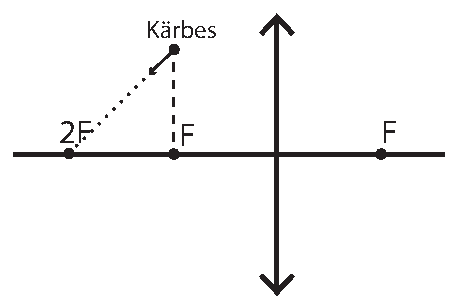
\includegraphics[width = 0.4\textwidth]{karbesjoonis.pdf}
	\end{center}
\end{wrapfigure}
\yl{KÄRBES}
Kärbes asub kumerläätse fokaaltasandil, läätse optilisest peateljest kaugusel $a = \SI{1}{m}$ ning hakkab lendama läätse kahekordse fookuskauguse suunas kiirusega $v = \SI{0,5}{m/s}$. Läätse fookuskaugus $f = \SI{1}{m}$. Millise kiirusega $u$ liigub kärbse kujutis sel hetkel, kui kärbse ja tema kujutise vaheline kaugus on minimaalne?
\punktid{6}\autor{Erkki Tempel}



\yl{2018}
Sul on kasutada takistid $R_1=\SI{10}{\ohm}$, $R_2=\SI{100}{\ohm}$ ning $R_3=\SI{1000}{\ohm}$. Kasutades ainult neid takisteid, mooodustage kuuest takistist koosnev süsteem nii, et kogutakistus oleks $R=\SI{2018}{\ohm}\pm\SI{0,2}{\ohm}$.
\punktid{6}\autor{Erkki Tempel}	



\yl{RING}
Traadist, mille ühe detsimeetri takistus on üks oom tehakse ring ümbermõõduga kuus detsimeetrit. Iga detsimeetri järel märgitakse punktid $a, b, \ldots, f$. Punktide $a$ ja $e$ vahele ühendatakse patarei pingega \SI{7}{V}, punktide $d$ ja $f$ vahele ampermeeter ning $d$ ja $b$ vahele voltmeeter. Punktid $f$ ja $b$ ühendatakse samast traadist lõigatud kahe-detsimeetrise traadijupiga. Leidke ampermeetri ja voltmeetri näidud.
\punktid{8}\autor{Jaan Kalda}



\yl{KAHURID}
Kahurist $A$ lastakse horisondi suhtes nurga $\alpha=\SI{30}{\degree}$ all lendu kuul algkiirusega $v_A=\SI{140}{m/s}$ kahuri $B$ suunas, mis on esimesest kahurist $l=\SI{1}{km}$ kaugusel samal tasapinnal. Sel hetkel, kui kuul on oma trajektoori kõrgeimas punktis, tulistatakse kahurist $B$ teine kuul, mis $t_1=\SI 5s$ pärast põrkub  esimese kuuliga. Millise algkiirusega tulistati kuul kahurist $B$? Õhutakistusega mitte arvestada; vabalangemise kiirendus $g\approx\SI{10}{m/s^2}$.
\punktid{8}\autor{Erkki Tempel}



\yl{HIIGLANE}
Jukul vanem vend on tema kaks korda suuremaks skaleeritud identne koopia. Kas vanem vend hüppab kõrgemale kui Juku? Eeldage, et hüppeliigutus on mõlemal juhul täpselt sama ja et lihaste poolt tekitatav jõud sõltub ainult lihaste ristlõikepindalast. Hüppe kõrguse saamiseks lahutame pealae kõrgusest hüppaja pikkuse.
\punktid{8}\autor{Andres Põldaru}
\pagebreak



\yl{MAGNETVÄLJAD}
Vaatleme prootoni liikumist x-y-tasandis. Vahemikus $0\leq x < \ell_1$ on magnetväli tugevusega $B$ z-telje positiivses suunas, vahemikus $\ell_1\leq x < \ell_1+\ell_2$ on magnetväli tugevusega $B$ z-telje negatiivses suunas. On teada, et $\ell_2 > \ell_1$. Ülejäänud tasandi osades magnetvälja pole. Alguses antakse prootonile mingi kiirus $\vec{v}$ tasandi vasakus pooles $x<0$. Milline on minimaalne kiirus $v=|\vec{v}|$, mille puhul saab valida sellise algse liikumissuuna, et prooton jõuab läbi kahe magnetväljaga vahemiku tasandi parempoolsesse osasse $x\geq \ell_1+\ell_2$? Prootoni laeng on $q$ ja mass on $m$.\punktid{10}\autor{Kaarel Hänni}

\begin{centering}
	
	\begin{tikzpicture}
	{
		\tikzset{ % This was originally used to update the global tikz style, but I prefer it to be locally defined instead
			odot/.style={
				circle,
				inner sep=0pt,
				node contents={$\odot$},
				scale=2
			},
			otimes/.style={
				circle,
				inner sep=0pt,
				node contents={$\otimes$},
				scale=2
			},
			circ/.style={
				circle,
				draw,
				minimum size=3mm,
				inner sep=0
			},
			odot2/.style={
				circ,
				path picture={\fill circle[radius=1pt];}
			},
			otimes2/.style={
				circ,
				path picture={
					\draw (path picture bounding box.45) -- (path picture bounding box.225);
					\draw (path picture bounding box.135) -- (path picture bounding box.315);
				}
			}
		}
		\draw[->] (-4,0) -- (4,0) node[below] {x};
		\draw[->] (-2,-2) -- (-2,3) node[left] {y};
		\draw (0,-2) -- (0,3);
		\draw (3,-2) -- (3,3);
		\draw[->] (-3.5,1) -- (-2.2,0.4) node[midway, below left] {$\vec{v}$};
		
		\draw [decorate,decoration={brace,amplitude=10pt}]
		(-2,0) -- (0,0) node [above, black,midway, yshift=7] {$\ell_1$}; 
		
		\draw [decorate,decoration={brace,amplitude=10pt}]
		(0,0) -- (3,0) node [above, black,midway, yshift=7] {$\ell_2$};
		
		\node [odot2] at (-1,2) {};
		\node [otimes2] at (1.5,2) {};
		\node at (-0.65,2) {$\vec{B}$};
		\node at (1.85,2) {$\vec{B}$};
	}
	\end{tikzpicture}
\end{centering}



\yl{KAUSS VEEGA}
Kaalul olevasse kaussi hakatakse ühtlaselt pudelist kõrgusel $h$ vett valama. Vee valamine lõpetatakse hetkel, mil kaalu näit on $m$. Mis on kaalu lugem $M$ peale stabiliserumist? Kas see on esialgsest näidust suurem, väiksem või võrdne? Õhutakistusega mitte arvestada.
\punktid{10}\autor{Krister Kasemaa}



\begin{wrapfigure}[6]{r}{0.4\textwidth}
	\vspace{-30pt}
	\begin{center}
		\hspace{-10pt}
		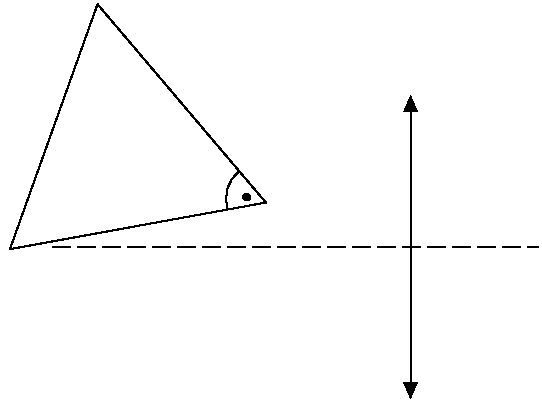
\includegraphics[width = 0.4\textwidth]{3nurk.pdf}
	\end{center}
\end{wrapfigure}
\yl{KOLMNURK}
Joonisel on kujutatud täisnurkse kolmnurga kujutis (täisnurk on märgitud punktiga) õhukeses läätses, mis on koos oma peateljega samuti ära näidatud. Konstrueerida kolmnurga täisnurkse tipu tegelik asukoht.
\punktid{12}\autor{Jaan Kalda}
\pagebreak



\begin{wrapfigure}[10]{r}{0.4\textwidth}
	\vspace{-20pt}
	\begin{center}
		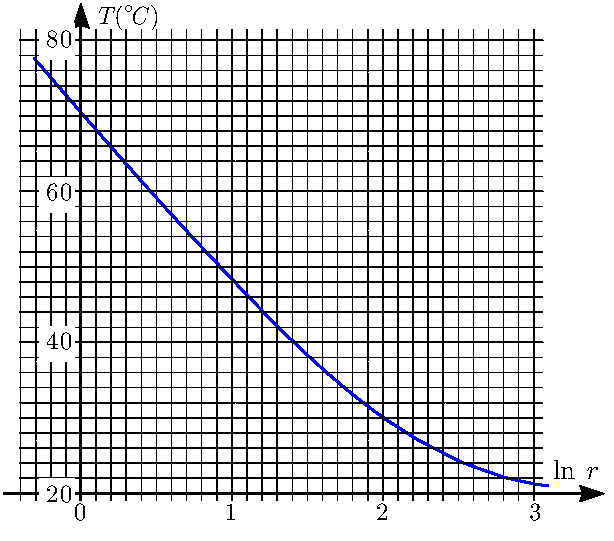
\includegraphics[width = 0.4\textwidth]{BesselK.pdf}
	\end{center}
\end{wrapfigure}

\yl{ÕHKJAHUTUS}\\
Valgusdiood tarbib elektrilist võimsust $P=\SI{50}W$. Dioodi jahutamiseks on see kinnitatud vaskplaadile paksusega $t=\SI{500}{\micro m}$. Vase soojusjuhtivustegur $k=\SI{385}{W/m.K}$. Juuresoleval graafikul (suuremalt lisalehel) on toodud plaadi temperatuur sõltuvuses vaadeldava punkti ja dioodi vahelise kauguse naturaallogaritmist. Kauguse mõõtmiseks kasutatud ühikud ei ole teada. Dioodi mõõtmed lugeda tühiselt väikseks. Milline on dioodi kasutegur (milline osa tarvitatud elektrienergiast kiirgub valgusenergiana)?

\textit{Märkus:} soojusjuhtivustegur on arvuliselt võrdne soojusenergiaga, mis kandub materjalis läbi ühikulise ristlõikepindala, kui temperatuur langeb ühe kraadi võrra ühe pikkusühiku kohta.
\punktid{12}\autor{Jaan Kalda}



\begin{wrapfigure}[7]{r}{0.4\textwidth}
	\vspace{-25pt}
	\begin{center}
		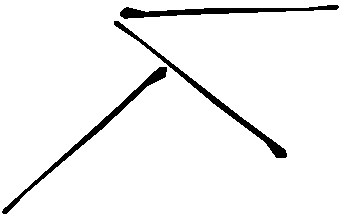
\includegraphics[width = 0.4\textwidth]{pulk.pdf}
	\end{center}
\end{wrapfigure}

\yl{PULK}
Õhkuvisatud pulga lendu filmiti liikumatu videokaamera abil ja kahe võrdse intervalli tagant võetud kolm kaadrit kopeeriti juuresolevale joonisele (suuremalt lisalehel). On teada, et esimese ja viimase kasutatud kaadri vahele jäänud ajavahemiku jooksul jäi pulga pöördenurk väiksemaks täispöördest. Pulk pöörles joonise tasandis, pulga pikkus oli $L=\SI{1.0}m$ ja kaadri lühem külg on täpselt vertikaalne; raskuskiirendus $g=\SI{9.8}{m/s^2}$. Kui kaugel pulga jämedamast otsast asub selle massikese? Kui pikk oli esimese ja viimase kaadri vaheline ajavahemik?
\punktid{14}\autor{Jaan Kalda}

\end{document}